\scanpage{118}
% archive foliation: 117
c) $\unsure2$ sommets d’ordre $2$
\figure{\begin{tikzpicture}[line cap=round,scale=.7]\draw(0,0)ellipse(.65 and.5);\fill(0,.5)circle(2pt);\fill(0,-.5)circle(2pt);\begin{scope}[shift={(3,0)}]\draw(-1,0)--(1,0);\fill(-.35,0)circle(2pt);\fill(.35,0)circle(2pt);\end{scope}\end{tikzpicture}}
d) $3$ sommets, dont deux d’ordre $1$, $1$ d’ordre $2$
\figure{\begin{tikzpicture}[line cap=round,scale=.7]\draw(-1,0)--(1,0);\foreach\a in{-1,0,1}\fill(\a,0)circle(2pt);\draw(-2,-.3)..controls(0,-.5)and(2,-1)..(4,1);\end{tikzpicture}}
\uline{degré $5$} \deleted{\unsure{4}}\quad a) $1$ sommet d’ordre $5$
\figure{\begin{tikzpicture}[line cap=round,scale=.7]\fill(0,0)circle(2pt);\draw(0,0)--(90:.65);\draw(0,0)--(162:.65);\draw(0,0)--(234:.65);\draw(0,0)--(306:.65);\draw(0,0)--(18:.65);\node at(-.8,.4){$\times$};\begin{scope}[shift={(3,1)}]\fill(0,0)circle(2pt);\draw(0,0)..controls(1.3,1.4)and(1.4,-1)..(0,0);\draw(-.7,.3)--(.5,-.1);\draw(-.6,-.3)--(0,0);\node at(.8,.1){$\times$};\end{scope}\begin{scope}[shift={(3,-0.4)}]\fill(0,0)circle(2pt);\draw(0,0)..controls(1.3,1.4)and(1.4,-1)..(0,0);\draw(-.7,.6)--(0,0)--(-.7,0);\draw(0,0)--(-.5,-.5);\node at(.6,.1){$\times$};\end{scope}\begin{scope}[shift={(5,-1)}]\fill(0,0)circle(2pt);\draw(0,0)..controls(-1.2,1.3)and(-1.5,-1.2)..(0,0)..controls(1.4,1.2)and(1.4,-1.2)..(0,0);\draw(0,0)--(.5,.1);\node at(1.4,0){$\times$};\end{scope}\begin{scope}[shift={(5,-2.1)}]\fill(0,0)circle(2pt);\draw(0,0)..controls(-1.2,1.3)and(-1.5,-1.2)..(0,0)..controls(1.4,1.2)and(1.4,-1.2)..(0,0);\draw(0,0)--(0,.5);\node at(1.4,0){$\times$};\end{scope}\end{tikzpicture}}
b) $2$ sommets, d’ordre $4$ et $1$
\figure{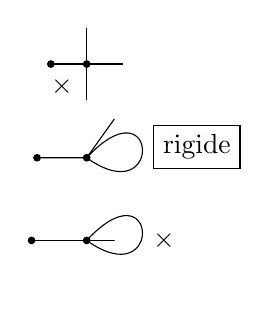
\begin{tikzpicture}[line cap=round,scale=.7]\fill(0,0)circle(2pt);\draw(0,0)--(90:.65);\draw(0,0)--(180:.65);\draw(0,0)--(270:.65);\draw(0,0)--(0:.65);\fill(-.65,0)circle(2pt);\node at(-.45,-.4){$\times$};\begin{scope}[shift={(0,-1.7)}]\fill(0,0)circle(2pt);\draw(0,0)..controls(1.3,1.4)and(1.4,-1)..(0,0);\draw(-.9,0)--(0,0)--(.5,.7);\fill(-.9,0)circle(2pt);\node[draw]at(2,.2){\uline{rigide}};\end{scope}\begin{scope}[shift={(0,-3.2)}]\fill(0,0)circle(2pt);\draw(0,0)..controls(1.3,1.4)and(1.4,-1)..(0,0);\draw(-1,0)--(.5,0);\fill(-1,0)circle(2pt);\node at(1.4,0){$\times$};\end{scope}\end{tikzpicture}}
c) $2$ sommets, d’ordre $3$ et $2$
\figure{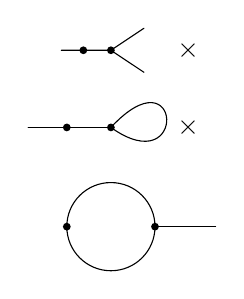
\begin{tikzpicture}[line cap=round,scale=.7]\fill(0,0)circle(2pt);\draw(-.9,0)--(0,0)--(.6,.4);\draw(0,0)--(.6,-.4);\fill(-.5,0)circle(2pt);\node at(1.4,0){$\times$};\begin{scope}[shift={(0,-1.4)}]\fill(0,0)circle(2pt);\draw(0,0)..controls(1.3,1.4)and(1.4,-1)..(0,0);\draw(-1.5,0)--(0,0);\fill(-.8,0)circle(2pt);\node at(1.4,0){$\times$};\end{scope}\begin{scope}[shift={(0,-3.2)}]\draw(0,0)circle(.8);\fill(-.8,0)circle(2pt);\fill(.8,0)circle(2pt);\draw(.8,0)--(1.9,0);\end{scope}\end{tikzpicture}}
d) $3$ sommets, dont $1$ d’ordre $3$, deux d’ordre $1$
\figure{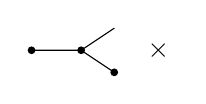
\begin{tikzpicture}[line cap=round,scale=.7]\fill(0,0)circle(2pt);\draw(-.9,0)--(0,0)--(.6,.4);\draw(0,0)--(.6,-.4);\fill(-.9,0)circle(2pt);\fill(.6,-.4)circle(2pt);\node at(1.4,0){$\times$};\end{tikzpicture}}
e) $3$ sommets, \deleted{dont} $2$ d’ordre $2$, $1$ d’ordre $1$
\deleted{\figure{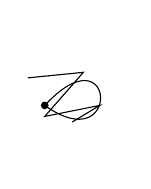
\begin{tikzpicture}[line cap=round,scale=.7]\fill(0,0)circle(2pt);\draw(0,0)..controls(1.3,1.4)and(1.4,-1)..(0,0);\draw(-.3,.5)--(.7,.6)--(0,-.2)--(1,0)--(.5,-.3);\end{tikzpicture}}}
\figure{\begin{tikzpicture}[line cap=round,scale=.7]\draw(-1,0)--(1.8,0);\foreach\a in{-1,0,1}\fill(\a,0)circle(2pt);\node at(2.3,0){$\times$};\end{tikzpicture}}
f) $4$ sommets, dont trois d’ordre $1$, $1$ d’ordre $2$\margin{impossible\ldots}
